\section{Grundlagen}

\subsection{Überblick}
Um unseren Lösungsansatz nachvollziehen zu können, ist es erforderlich, 
die Problemstellung detailliert zu analysieren. Im ersten Schritt wird betrachtet, 
welche Zielgruppe Ludwig System anspricht und welche spezifischen Optimierungen 
das Unternehmen verfolgt. Im Anschluss werden bestehende Lösungsansätze verglichen, 
um deren Stärken und Schwächen zu bewerten und als Grundlage 
für die Entwicklung eines verbesserten Systems zu nutzen.



\subsubsection{Anwendungsdomäne}
Das Abhängen von Lasten per Hand ist nicht nur zeitaufwendig, sondern oft auch gefährlich. 
Ludwig System bietet mit ihren funkgesteuerten Lasthaken eine innovative Lösung, 
die diese Arbeit deutlich erleichtert. Diese Haken ermöglichen es den Mitarbeitenden, 
Lasten aus sicherer Entfernung anzuheben und auszubalancieren. Besonders beliebt ist 
die Traverse, die speziell für den Transport von Dachelementen und Wänden entwickelt wurde. 
Allerdings müssen aktuelle Versionen noch manuell an die Last befestigt werden, 
was besonders bei hohen Wänden zeitaufwendig und gefährlich sein kann. 
Abbildung 2.2 illustriert die Nutzung der Traverse beim Transport eines Dachelements.


\begin{figure}[H]
    \centering
    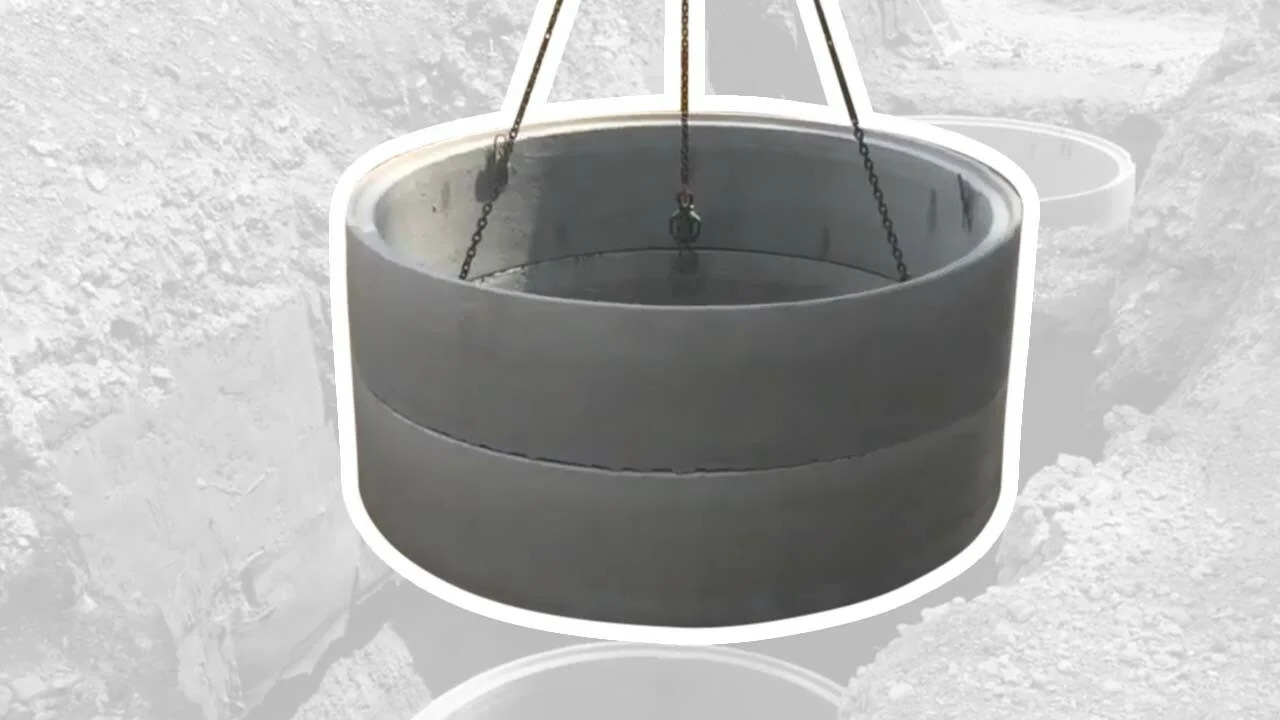
\includegraphics[width=0.5\textwidth]{graphics/Betonelement.jpg}\hfill%
    \caption{Ludwig Hook mit Betonelement}
    \centering
    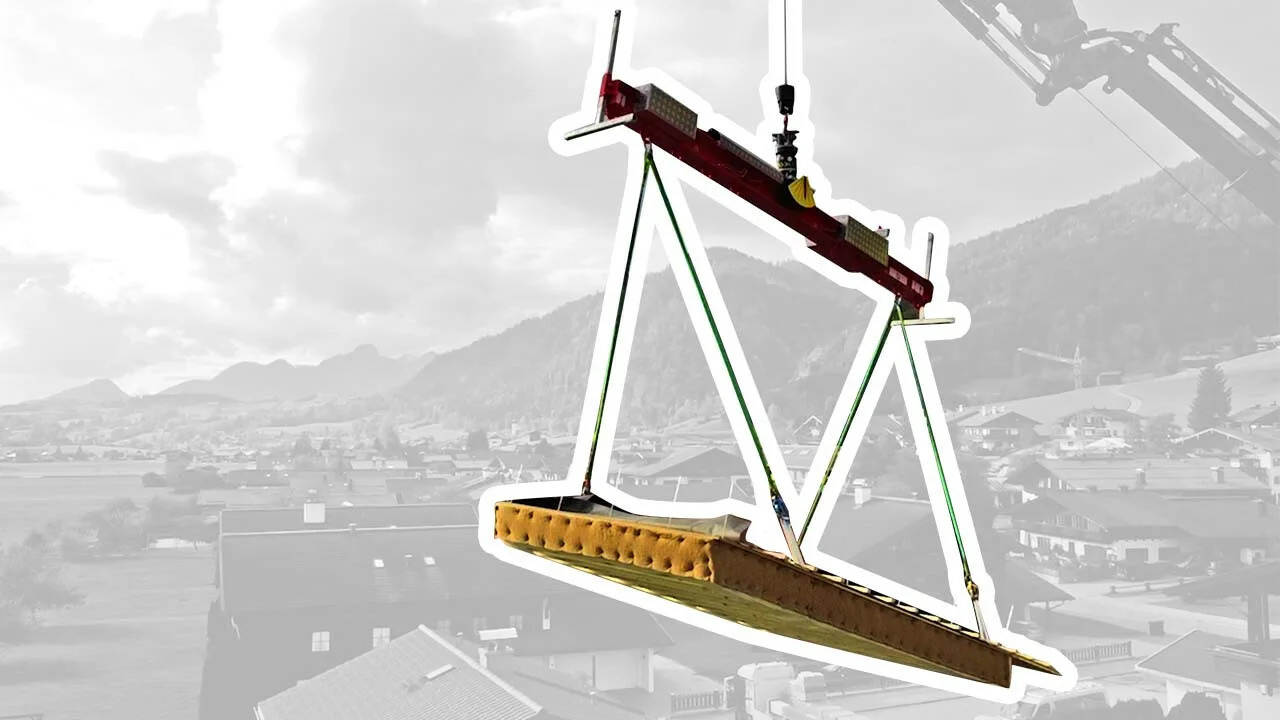
\includegraphics[width=0.5\textwidth]{graphics/Traverse.jpg}
    \caption{Traverse mit Dachelement}
\end{figure}

\subsubsection{Last}
Unter Lasten sind vor allem Fertigstrukturen wie z.B. Fertig erstellte Wände oder Dächer. Lasten haben maximal 2 Anschlagspunkte, welche einen Abstand von 1m bis 6m zueinander haben. Diese Anschlagspunkte können auf unterschiedliche Höchen sein, wie z.B. bei Dächer welche eine Neigung besitzen.


\clearpage
\subsubsection{Traverse}
Die LudwigTraverse ist eine Spezialtraverse, die speziell für den Lastausgleich entwickelt 
wurde. Sie erweist sich insbesondere dann als nützlich, wenn die Anschlagpunkte 
falsch positioniert sind und dadurch der Schwerpunkt der Last nicht korrekt berücksichtigt wird. 
Dies kann zu einer schrägen Ausrichtung beim Anheben der Last führen \cite{ludwigTraverse}.

\begin{figure}[H]
    \centering
    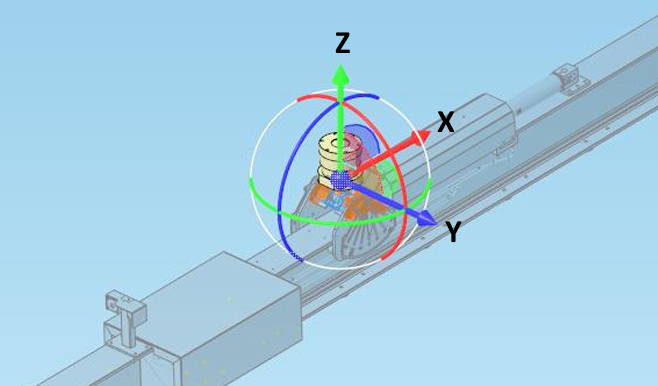
\includegraphics[width=0.5\linewidth]{graphics/Traverse_Rotationen.PNG}
    \caption{Koordinaten-System der Ludwig System Traverse}
    \label{fig:traverse}
\end{figure}

Abbildung \ref{fig:traverse} zeigt das linkshändige Koordinaten-System der Traverse.
Die Traverse hat Dimensionen (Länge × Breite y Höhe z) von 500 cm × 70 cm × 50 cm.
Dabei wird fortan die Rotation um die Y-Achse der Traverse als Neigen definiert und die Rotation 
um die Z-Achse der Traverse, als Rotieren definiert.


\subsection{Stand der Forschung}

\subsubsection{Arbeit: Objekterkennung und Distanzmessung für KollisionsVermeidung bei Lastenhebung}
(Arbeit: Object Detection and Distance Measurement Algorithm for Collision Avoidance of Precast Concrete Installation during Crane Lifting Process\cite{yong_object_2023} Erklären)

\subsubsection{Arbeit: Objekterkennung und 3D-basierte Objektortung für automatische Lastenhebung}
(Arbeit: Image-based onsite object recognition for automatic crane lifting tasks\cite{zhou_image-based_2021} Erklären)

\subsubsection{Arbeit: Erkennung von auf Robotersystemen angebrachten Passermarken}


\subsection{Passermarker}
Passermarker sind ein essenzielles Werkzeug in der modernen Bildverarbeitung und spielen eine 
zentrale Rolle in der räumlichen Orientierung und Positionsbestimmung. Insbesondere in Anwendungen 
wie der automatisierten Lastenhebung, wie sie von Ludwig System angestrebt wird, können Passermarker 
helfen, Anschlagpunkte präzise zu lokalisieren.

Diese Marker, darunter Barcodes, QR-Codes oder speziell entwickelte AR-Marker, liefern visuelle 
Referenzen, die von Kamerasystemen erkannt und interpretiert werden können. Damit ermöglichen sie es, 
Objekte im Raum genau zu positionieren oder auszurichten.

In diesem Abschnitt untersuchen wir die Grundlagen von Passermarkern und beleuchten ihre spezifischen 
Einsatzmöglichkeiten in unserem Szenario, insbesondere im Kontext der automatisierten Ausrichtung von 
Anschlagpunkten auf der Traverse.

\subsubsection{Einführung Passermarker}
Passermarker sind quadratische Muster, die auf flachen Oberflächen aufgedruckt werden. 
Sie dienen als visuelle Referenzpunkte, die von Kamerasystemen erkannt und interpretiert 
werden können. Es gibt verschiedene Arten von Passermarkern, die je nach Anwendung 
unterschiedliche Eigenschaften und Einsatzmöglichkeiten bieten. 
Abbildung \ref{fig:marker_types} zeigt eine Auswahl solcher Marker.

\begin{figure}[H]
    \centering
    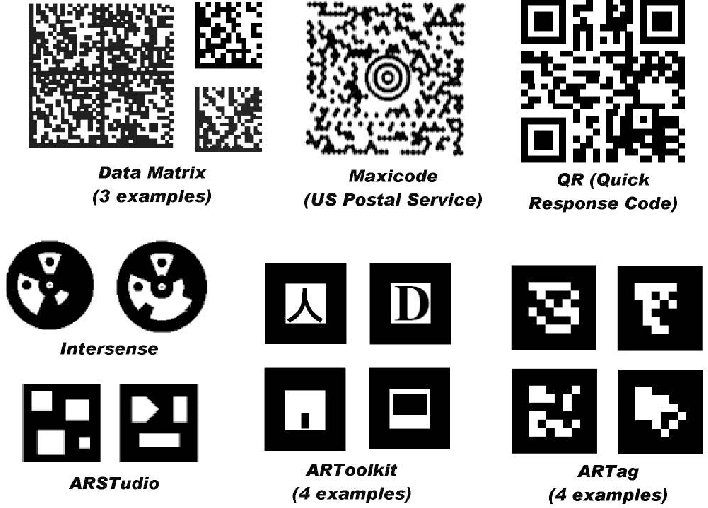
\includegraphics[width=0.5\linewidth]{graphics/marker_arten.png}
    \caption{Verschiedene Marker Arten}
    \label{fig:marker_types}
\end{figure}

Grundsätzlich gilt: Je komplexer und größer ein Marker ist, desto mehr Informationen können
darin gespeichert werden. Dabei muss jedoch der Informationsgehalt immer an die spezifischen 
Anforderungen der Anwendung angepasst werden, um eine optimale Balance zwischen Größe, Lesbarkeit 
und Informationsdichte zu gewährleisten.

In der Robotik gehören AprilTags und AruCo-Marker zu den meistgenutzten Passermarkern. 
Ihre Beliebtheit basiert auf ihrer Robustheit und Effizienz bei der Lokalisierung in 
dreidimensionalen Räumen. Diese Marker wurden speziell entwickelt, um Verzerrungen und 
schwierige Lichtverhältnisse zu kompensieren und eine präzise Posenschätzung zu ermöglichen. 
Ihre Anwendung wird im weiteren Verlauf dieser Arbeit genauer beleuchtet, insbesondere im 
Kontext der automatisierten Lokalisierung von Anschlagpunkten.


\subsubsection{Posenschätzung durch AR Marker}


\subsubsection{Probleme mit Passermarkern}



\subsection{Objekterkennung durch Machine Learning}
\subsubsection{Grundlagen Objekterkennung mit Neuronalen Netzen}
\subsubsection{Vorhandene Modelle}
\subsubsection{Probleme mit Machine Learning}


\subsection{Kameras}
\subsubsection{Kameraeigenschaften}
(Erklären was FOV, Verzerrrungen etc ist)
\subsubsection{Intrinsische Kalibrierung}
\subsubsection{Herausforderungen}

\subsection{Vorhandene Frameworks}
(Erklärung von OpenCV und ihren Methoden)

